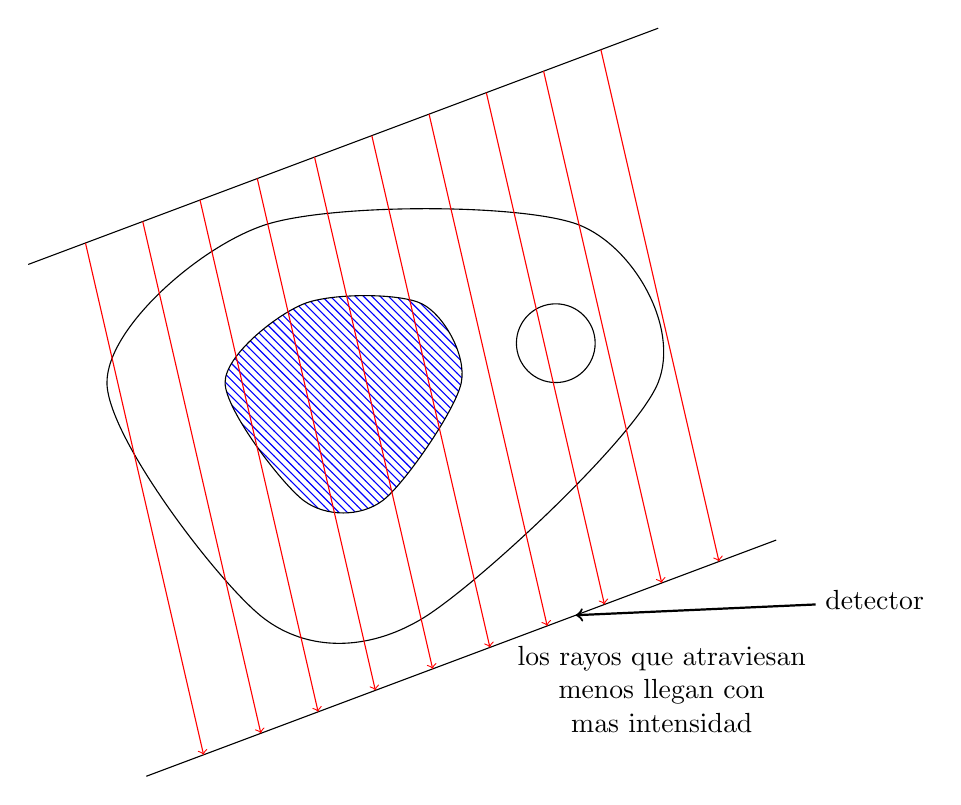
\begin{tikzpicture}

	\usetikzlibrary{patterns}

	\draw plot[smooth cycle]
	coordinates {(-3,0) (-1,-3) (1,-3) (4,0) (3,2) (-1,2)};
	
	\draw[pattern=north west lines, pattern color=blue] plot[smooth cycle]
	coordinates {(-3/2,0) (-1/2,-3/2) (1/2,-3/2) (3/2,0) (2/2,2/2) (-1/2,2/2)};
	\draw (2.7,0.5) circle (0.5cm) ;
	
	\draw (-4,1.5) -- (4,4.5);
	
	\draw (-2.5,-5) -- (5.5,-2);
	
	\foreach \x in {1,...,10}
	{\draw[->,red]
		(\x/11*8-4,\x/11*3+1.5) -- (\x/11*8-2.5,\x/11*3-5);
	}
	
	\draw[->, thick]
		(6,8/11*3-5) -- (7.5/11*8-2.5,7.5/11*3-5);
		
	\node at (6,8.2/11*3-5) [right] {detector};
	
	\node at (9/11*8-2.5,6.5/11*3-5) [below, text width=4cm, align=center] {los rayos que atraviesan menos llegan con mas intensidad};


\end{tikzpicture}